\begin{sepframe}{Introduction}
    {\scriptsize{If you can't explain it simply, you don't understand it well enough.}}
\end{sepframe}

\begin{frame}[fragile,c]
    \frametitle{Composition and inheritance}
    \framesubtitle{Map}

    \makebox[\linewidth]{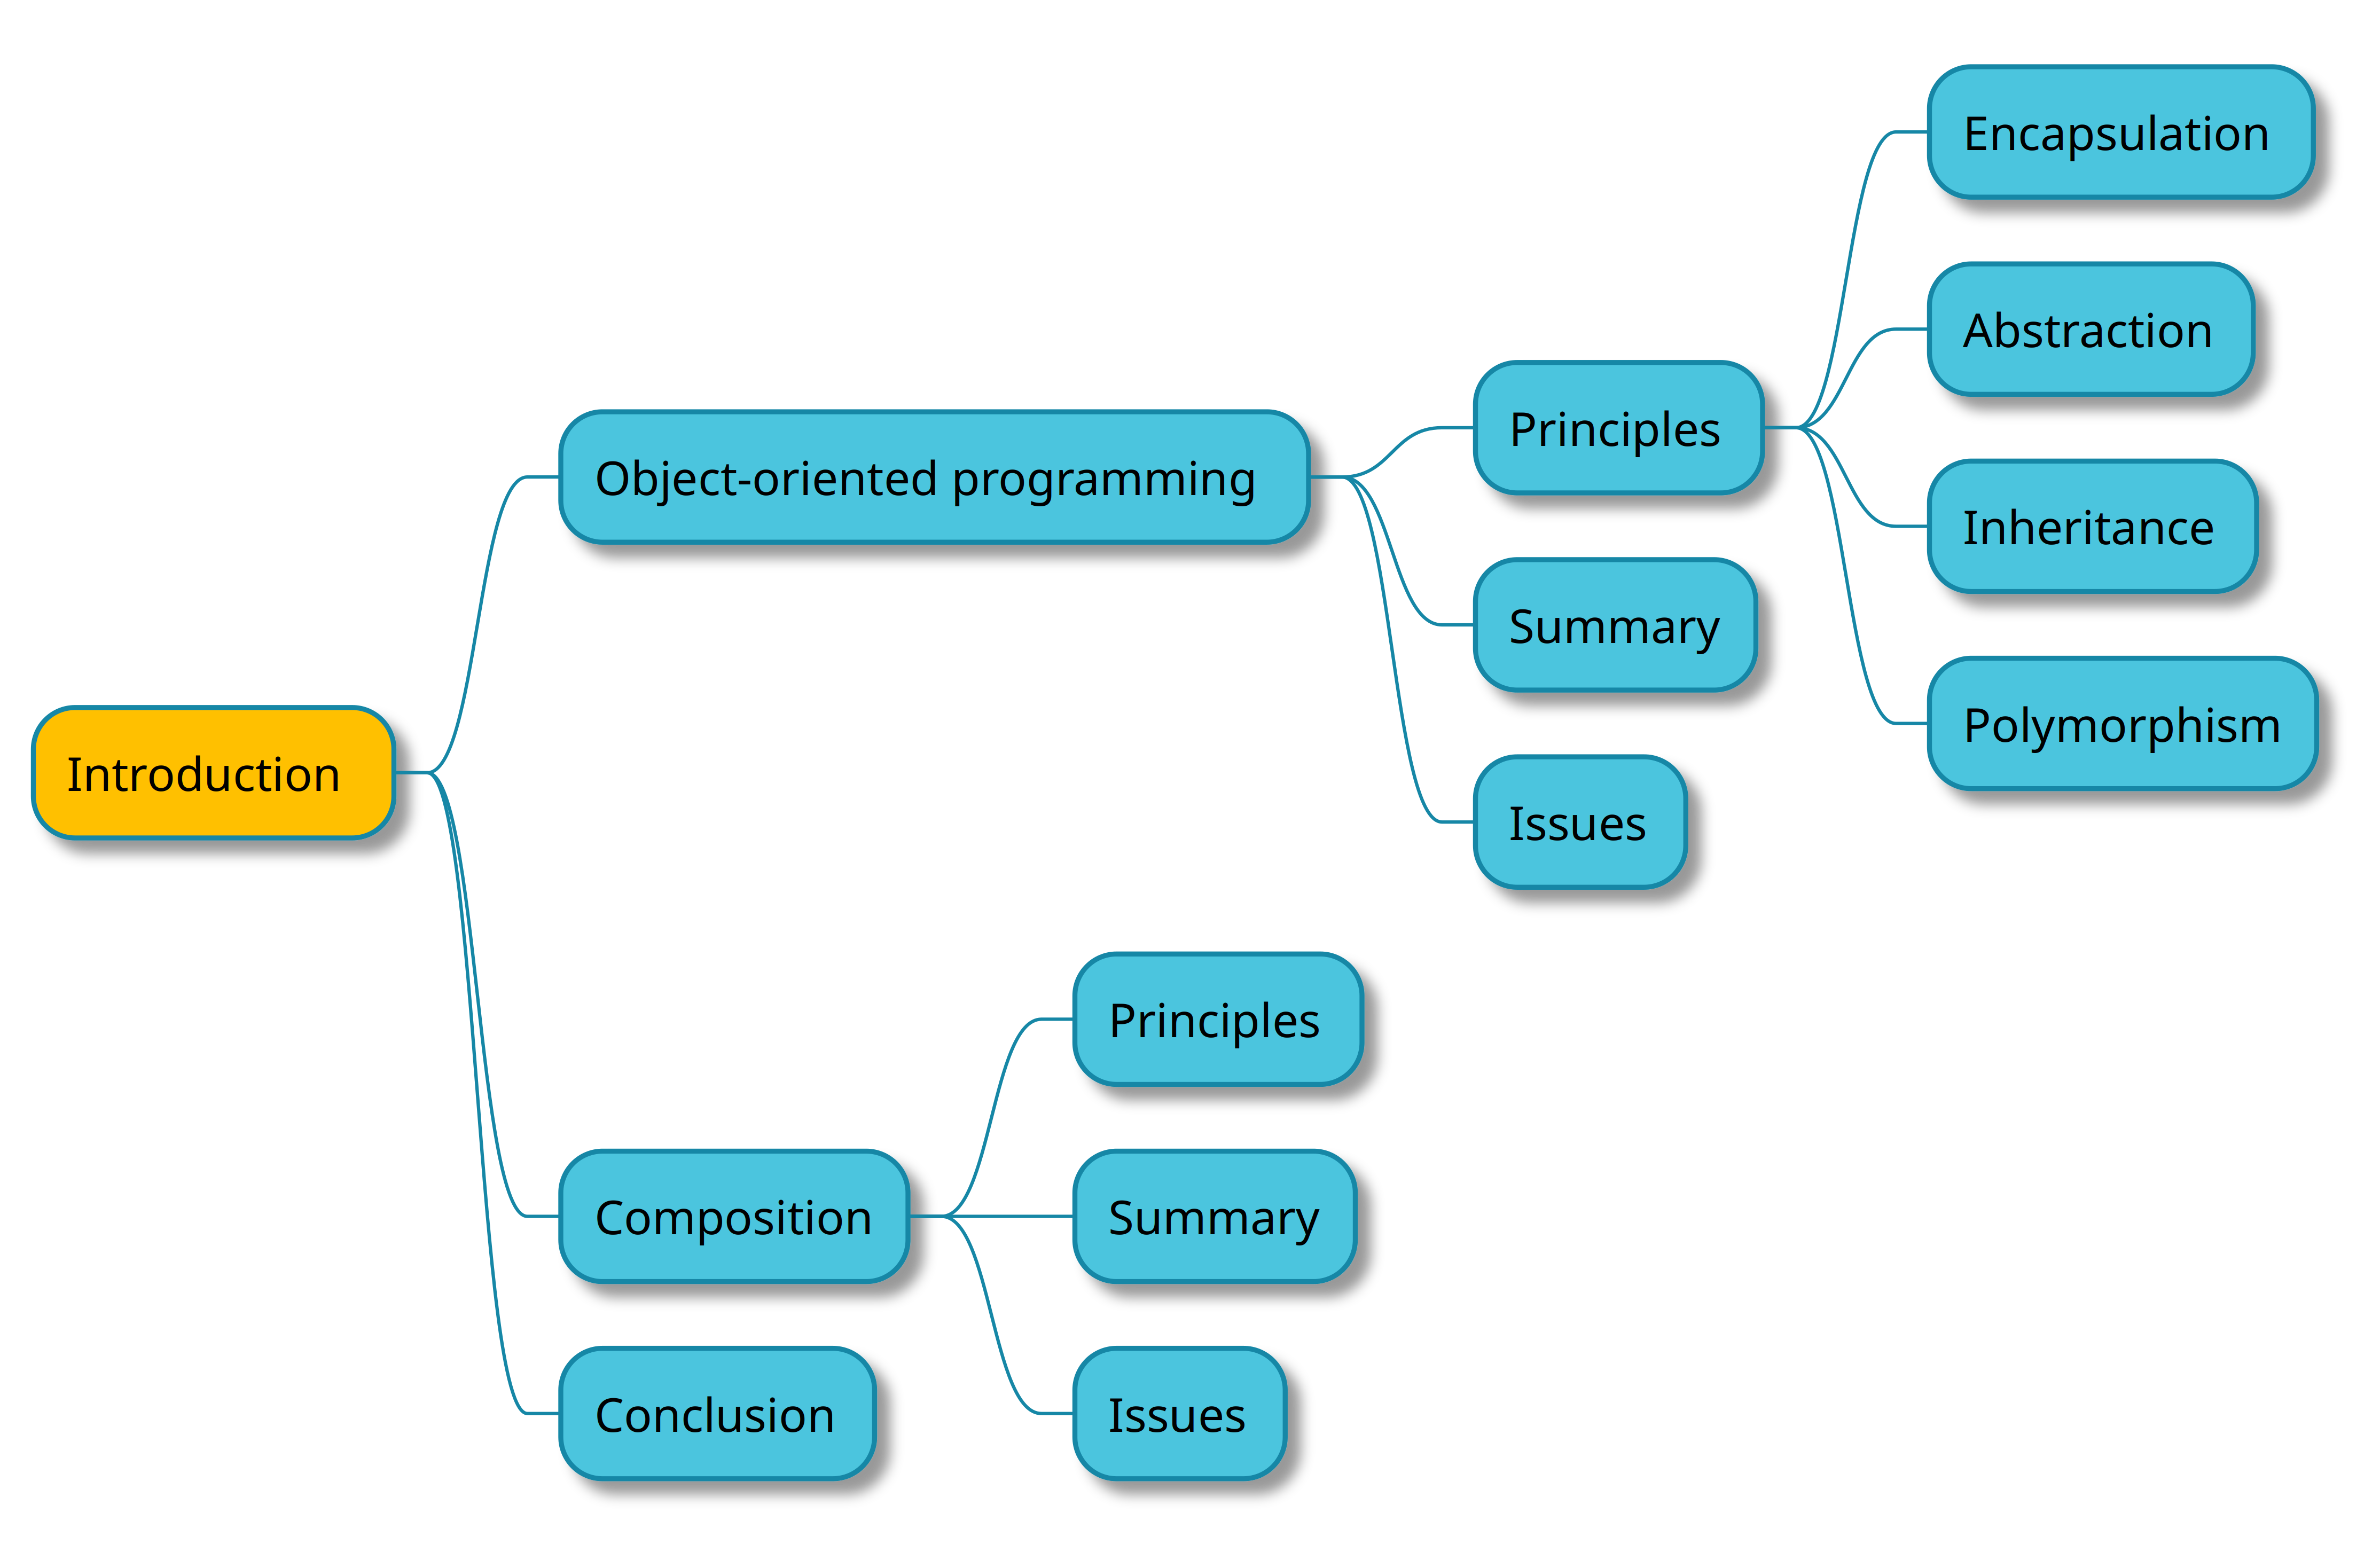
\includegraphics[width=\paperwidth]{src/session--composition-and-inheritance/resources/summary.png}}
\end{frame}

\begin{frame}
    \frametitle{Introduction}

    Inheritance and composition are two programming paradigms developers use to establish
    relationships between classes and objects.
\end{frame}

\begin{frame}
    \frametitle{Introduction}

    Whereas \textbf{inheritance} derives one class from another, \textbf{composition} defines
    a class as the sum of its parts.
\end{frame}

\begin{frame}
    \frametitle{Introduction}

    Classes and objects created through \textbf{inheritance} are tightly coupled because
    changing the parent or superclass in an inheritance relationship risks breaking your code.\\~\\

    \pause

    Classes and objects created through \textbf{composition} are loosely coupled, meaning
    that you can more easily change the component parts without breaking your code.
\end{frame}

\begin{frame}
    \frametitle{Introduction}
    Because loosely coupled code offers more flexibility, many developers have learned that
    \textbf{composition} is a better technique than \textbf{inheritance}.
\end{frame}

\begin{frame}[c]
    \begin{center}
        \Huge At which cost?
    \end{center}
\end{frame}
